%%%%%%%%%%%%%%%%%%%%%%%%%%%%%%%%%%
\section{Introduction}
%%%%%%%%%%%%%%%%%%%%%%%%%%%%%%%%%%

%A significant fraction of proton--proton ($pp$) collisions at the LHC involves quasi-real photon interactions.
Precise calculations of various electroweak reactions in $pp$ collisions at the LHC need to account for, on top of the higher-order corrections, the effects of photon-induced subprocesses.
The relevant examples are the production of lepton pairs~\cite{Aad:2014qja, Aad:2016zzw,Accomando:2016tah, Luszczak:2015aoa, Harland-Lang:2016apc} or pairs of electroweak bosons~\cite{Luszczak:2014mta, Denner:2015fca, Dyndal:2015hrp, Ababekri:2016kkj, Biedermann:2016guo, Biedermann:2016yvs, Yong:2016njr, Luszczak:2018ntp}.


Recently, a precise photon distribution inside the proton has been evaluated in Ref.~\cite{Manohar:2016nzj}.
This approach provides a model-independent determination of the photon PDF (embedded in so-called LUXqed distribution)
and  it is based on proton structure function and elastic form factor fits in electron--proton scattering.

Up to date, there are no experimentally clean processes identified that would allow to either strongly constrain or verify the calculations.
For example, the extraction of photon PDF from isolated photon production in deep inelastic scattering (DIS)~\cite{Schmidt:2015zda} 
or from inclusive $pp\rightarrow\ell^+\ell^-+X$ reaction~\cite{Ball:2013hta, Aad:2016zzw, Giuli:2017oii} is limited due to large QCD background.
On contrary, the elastic part of the photon PDF is verified via exclusive $\gamma\gamma\rightarrow\ell^+\ell^-$ process, measured in $pp$ collisions by ATLAS~\cite{Aad:2015bwa,Aaboud:2017oiq}, CMS~\cite{Chatrchyan:2011ci,Chatrchyan:2012tv} and recently by CMS+TOTEM~\cite{Cms:2018het} collaborations.




We therefore propose a new experimental method to constrain photonic content of the proton.
Thanks to the large fluxes of quasi-real photons from the Pb ion at the LHC, the photon-induced dilepton production in $p+\textrm{Pb}$ collision configuration is a very clean way to probe photon PDF.
This process is shown schematically in Fig.~\ref{fig:diagrams}, where by analogy to DIS, two leading-order diagrams can be identified.
Since the photon flux from the ion scales with $Z^2$ and QCD-induced cross-sections scale approximately with $A$,
the amount of QCD background is greatly reduced comparing to $pp$ case.

\begin{figure}[h!]
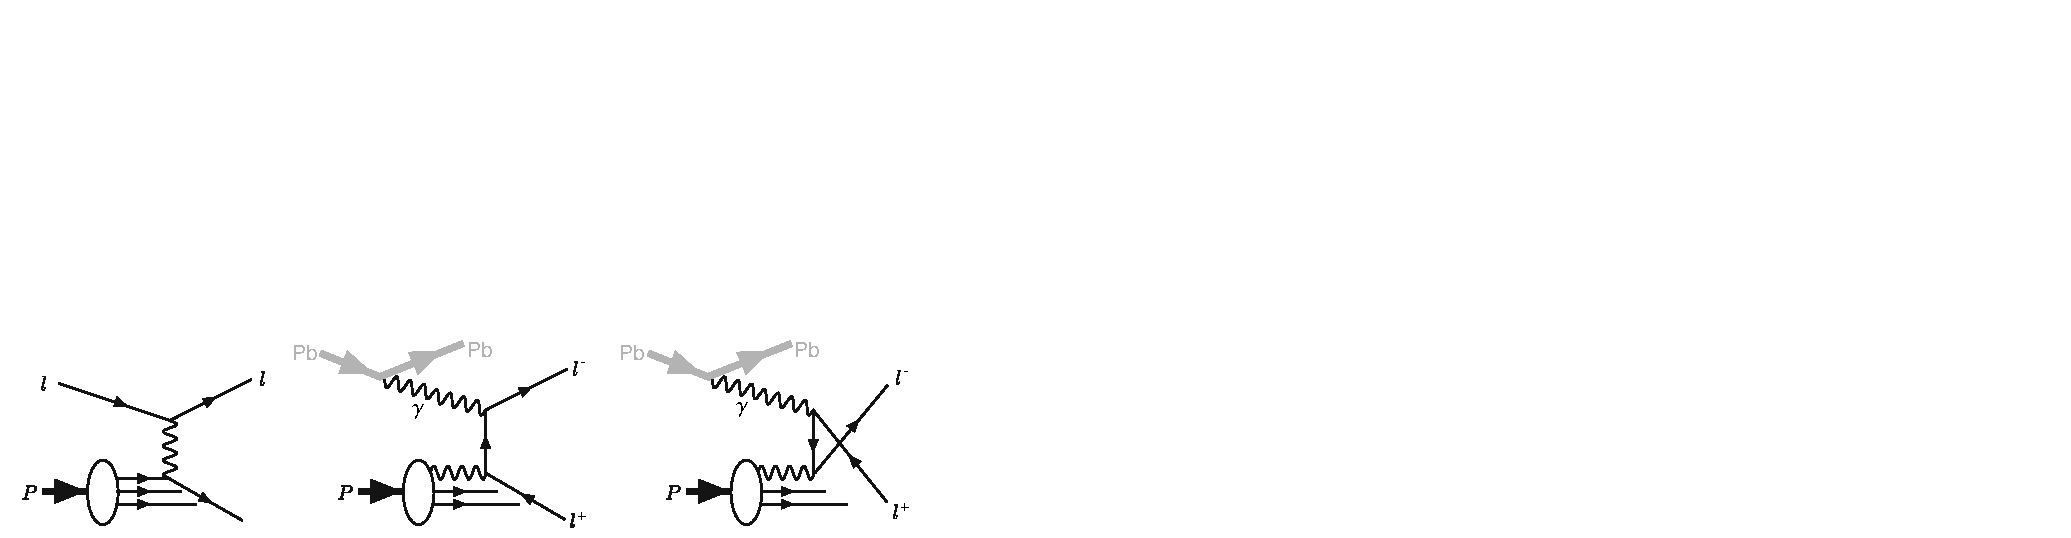
\includegraphics[width=1.\textwidth]{figures/dis_to_photon_v2.pdf}
 \put(-400,-3){{\footnotesize(a)}}
 \put(-246,-3){{\footnotesize(b)}}
\put(-90,-3){{\footnotesize(c)}}
\caption{Schematic graphs for deep inelastic scattering, $\ell^{\pm} p\rightarrow \ell^{\pm} +X$ (a) and photon-induced dilepton prodcution, $\gamma p\rightarrow \ell^+\ell^- + X$, in $p+\textrm{Pb}$ collisions for $t$-channel (b) and $u$-channel (c) lepton exchange.}
\label{fig:diagrams}
\end{figure}

Moreover, as this process does not involve the exchange of color with the photon-emitting nucleus, no significant particle production is expected in the rapidity region between the dilepton system and the nucleus. 
The photon-emitting nucleus is also expected to produce no neutrons because the photons couple to the entire nucleus. 
Thus, a combination of a rapidity gap and zero neutrons in the same direction provide straightforward criteria to identify these events experimentally. 



